%Lineare Regression
Mete O.~Rologe beobachtet mit Sorge, wie sich während eines Schneefalls
die Temperatur entwickelt:
\begin{center}
\begin{tabular}{|c|c|}
\hline
Zeit&Temperatur\\
\hline
\phantom{0}8&$-0.5^\circ \text{C}$\\
\phantom{0}9&$\phantom{-}0.1^\circ \text{C}$\\ 
10&$\phantom{-}1.1^\circ \text{C}$\\
11&$\phantom{-}3.0^\circ \text{C}$\\
\hline
\end{tabular}
\end{center}
Mete weiss, dass es zu regnen beginnen wird, wenn die Temperatur über
$4^\circ\text{C}$ ansteigt.
Er versucht daher mit Hilfe eines linearen Modells den Zeitpunkt 
vorherzusagen, wann die Temperatur $4^\circ \text{C}$ sein wird.
\begin{teilaufgaben}
\item
Wann wird die Temperatur $4^\circ \text{C}$ erreichen?
\item
Ist das lineare Modell eine zweckmässige Approximation des tatsächlichen
Geschehens?
\end{teilaufgaben}

\thema{lineare Regression}

\begin{loesung}
\begin{figure}
\centering
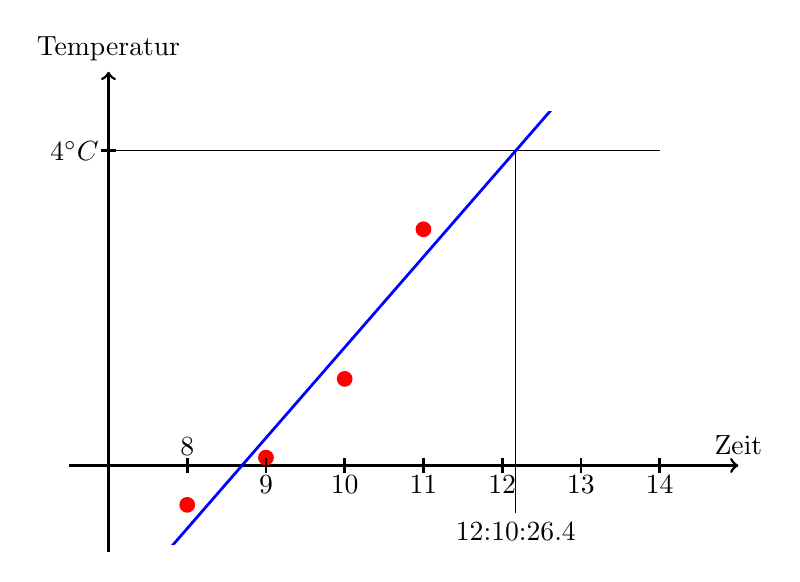
\begin{tikzpicture}[scale=1]
\draw[->,line width=1pt] (6.5,0)--(15,0) coordinate[label=Zeit];
\draw[->,line width=1pt] (7,-1.1)--(7,5) coordinate[label=Temperatur];
\fill[color=red] (8,-0.5) circle[radius=0.1];
\fill[color=red] (9,0.1) circle[radius=0.1];
\fill[color=red] (10,1.1) circle[radius=0.1];
\fill[color=red] (11,3.0) circle[radius=0.1];
\draw (7,4)--(14,4);
\draw[line width=1pt] (8,-0.1)--(8,0.1);
\draw[line width=1pt] (9,-0.1)--(9,0.1);
\draw[line width=1pt] (10,-0.1)--(10,0.1);
\draw[line width=1pt] (11,-0.1)--(11,0.1);
\draw[line width=1pt] (12,-0.1)--(12,0.1);
\draw[line width=1pt] (13,-0.1)--(13,0.1);
\draw[line width=1pt] (14,-0.1)--(14,0.1);
\draw[line width=1pt] (6.9,4)--(7.1,4);
\draw (12.174,-0.6)--(12.174,4);
\node at (12.174,-0.6) [below] {12:10:26.4};
\node at (7,4) [left] {$4^\circ\text{C}$};
\node at (8,0) [above] {$8$};
\node at (9,0) [below] {$9$};
\node at (10,0) [below] {$10$};
\node at (11,0) [below] {$11$};
\node at (12,0) [below] {$12$};
\node at (13,0) [below] {$13$};
\node at (14,0) [below] {$14$};
\begin{scope}
\clip (7,-1) rectangle (15,4.5);
\draw[color=blue,line width=1pt] (7,-1.95)--(15,7.25);
\end{scope}
\end{tikzpicture}
\caption{Abhängigkeit von Temperatur und Zeit in Aufgabe~\ref{40000042}.
\label{40000042:graph}}
\end{figure}
%
Wir führen lineare Regression für die gegebenen Daten durch:
\begin{center}
\begin{tabular}{|
>{$}c<{$}|
>{$}r<{$}
>{$}r<{$}|
>{$}r<{$}
>{$}r<{$}
>{$}r<{$}|}
\hline
i& X&   Y&X^2&  Y^2&   XY\\
\hline
1& 8&-0.5& 64& 0.25& -4.0\\
2& 9& 0.1& 81& 0.01&  0.9\\
3&10& 1.1&100& 1.21& 11.0\\
4&11& 3.0&121& 9.00& 33.0\\
\hline
\Sigma
 &38& 3.7&366&10.47& 40.9\\
\hline
\end{tabular}
\end{center}
Daraus können wir die Regressionsgerade und den Regressionskoeffizienten
berechnen:
\begin{align*}
a
&=
\frac{4\cdot 40.9 - 38\cdot 3.7}{4\cdot 366 - 38^2}
=
\frac{23}{20}
=
1.15
\\
b
&=
\frac14\cdot 3.7 -a\frac14\cdot 38
=
-10
\\
r^2
&=
\frac{(4\cdot 40.9 - 38\cdot 3.7)^2}{
(4\cdot 366-38^2)(4\cdot 10.47-3.7^2)
}
=
\frac{23^2}{20\cdot 28.19}
=
0.93828
\\
r&=0.96865
\end{align*}
\begin{teilaufgaben}
\item
Der Zeitpunkt, zu dem die Temperatur $4^\circ\text{C}$
erreicht, ist Lösung der Gleichung
\[
4=aX+b
\qquad\Rightarrow\qquad
X
=
\frac{4-b}{a}
=
12.174,
\]
also um 12:10:26.4.
\item
Der Regressionskoeffizient $r^2$ ist relativ nahe bei $1$ und daher
ist die Regeression wohl ein eingermassen gut geeignetes Modell.
\end{teilaufgaben}
Die Regressionsgerade ist in Abbildung~\ref{40000042:graph} dargestellt.
\end{loesung}

\begin{bewertung}
Lineare Regression ({\bf L}) 1 Punkt,
Berechnung von $a$ ({\bf A}) und $b$ ({\bf B}) je 1 Punkt,
Bestimmung des Zeitpunkts ({\bf Z}) 1 Punkt,
Berechnung von $r^2$ ({\bf R}) 1 Punkt,
Qualitätsbeurteilung mit Hilfe von $r^2$ ({\bf Q}) 1 Punkt.
\end{bewertung}
